%Started on Friday, 11 August 2006
%Aug: 23, 29, 30, 31
%Sep:  1
% 2007
%Jan: 16, 17, 22
%Feb:  6,  9, 11, 22
%Mar:  8, 20, 21, 22, 27, 28, 29, 30, 31
%Apr:  1,  2,  3, 11, 18
%May:  2,  3,  4,  6,  7,  8, 10, 11, 12, 13, 14
%Sep: 18, 19

%
% Chapter: 
%
\label{ch:Correctors}

In this chapter we first discuss subspace searches as a way 
to determine search directions for interior point methods
for linear programming.
Then we illustrate the theoretical understanding of 
the cases of failure of Mehrotra's corrector direction,
drawing particularly from \cite{Cartis04,Cartis05}, 
and we introduce a computationally competitive way
to improve the performance of multiple centrality correctors.
We present the implementation of such a strategy in the \HOPDM solver,
along with extensive computational experience.
The original content of this chapter has already appeared 
in \cite{ColomboGondzio05}, co-authored with Jacek Gondzio.


%
% Section
%
\section{Subspace searches}
\label{sec:SubspaceSearches}

Subspace searches are a strategy for generating search 
directions. 
They are usually derived differently than the Newton system, and 
are built according to some criteria that are believed to summarise
the essential characteristics of a good search direction.
In this section we discuss two subspace-search approaches. 
The first, by Jarre and Wechs \cite{JarreWechs}, generates directions
by a recursion on a modification of Mehrotra's corrector.
The second, the approach of Mehrotra and Li \cite{MehrotraLi},
considers search directions
produced through Krylov subspace basis.

%
%
\subsection{Jarre and Wechs's directions}
\label{sec:JarreWechs}

Jarre and Wechs \cite{JarreWechs} % took a more pragmatic view and
present an implementable technique for generating efficient 
higher-order search directions in a primal--dual interior-point framework.
They start by considering the Newton system (\ref{eq:NewtonSystem}).
While it is clear what to consider as right-hand 
side for primal and dual feasibility constraints (the residual 
at the current point), the complementarity component leaves more 
freedom in choosing a target $t$. They argue that there exists 
an optimal choice for which the corresponding Newton system would 
immediately produce the optimizer.
Given the system
\be
\label{eq:JarreWechsSystem}
\left[ \begin{array}{ccc}
    A & 0   & 0 \\
    0 & A^T & I \\
    S & 0   & X
  \end{array} \right]
\left[ \begin{array}{c}
    \Delta x \\ \Delta y \\ \Delta s
  \end{array} \right] =
\left[ \begin{array}{c}
    b-Ax \\ c-A^Ty-s \\ t
  \end{array} \right],
\ee
they ask what choice of $t$ in the right-hand side 
would produce a good search direction.

If $w$ is the current iterate and 
$w^*$ is an optimal primal--dual solution to 
problem (\ref{eq:PrimalDualPair}), then 
$\Delta w^*= w^*-w$ satisfies the 
system (\ref{eq:JarreWechsSystem}) for the choice
\be  \label{eq:OptimalTarget}
  t^* = S(x^*-x) + X(s^*-s) = S\Delta x^* + X\Delta s^*.
\ee
It is possible to write $t^*$ as a different expression. 
Given that $X^*S^*e=0$, we have:
\[
  0 = (X+\Delta X^*)(S+\Delta S^*)e 
    = XSe + X\Delta s^* +S\Delta x^* +\Delta X^*\Delta S^*e,
\]
from which, using (\ref{eq:OptimalTarget}), we obtain
$t^* = -XSe - \Delta X^* \Delta S^*e$.
Therefore, as $t^*$ would lead to the optimizer in one single iteration,
it can be considered the optimal choice for the target $t$
in (\ref{eq:JarreWechsSystem}).

Clearly, as we do not know what the solution will be,
when system (\ref{eq:JarreWechsSystem}) is set up, 
we have no knowledge of $t^*$. 
However, some bounds can be determined. Knowing that 
$x+\Delta x^* \ge 0$ and $s+\Delta s^* \ge 0$, we have 
$\Delta x^* \ge -x$ and $\Delta s^* \ge -s$, from which we obtain
the lower bound
\[
  t^*= S\Delta x^* + X\Delta s^* \ge -2XSe.
\]

\ignore{
It would be interesting to see if in practice this bound is useful. 
We could check whether at any iteration it's violated, and if so just
put the bound...
}

An upper bound is derived from a result by Vavasis and Ye 
\cite[Lemma~16]{VavasisYe}, which states that for two 
strictly feasible points, $w$ and $\hat w$, exactly on the central path
and $\mu > \hat\mu > 0$ we have
\[
  s_i \hat x_i + x_i \hat s_i \le n x_i s_i, \qquad i = 1, \ldots, n,
\]
which can be written in vector terms as
\be  \label{eq:UpperBound}
  S\hat Xe + X \hat Se \le nXSe.
\ee
Therefore, thanks to (\ref{eq:UpperBound}) 
we can rewrite (\ref{eq:OptimalTarget}) and derive the following upper bound:
\[
  t^*= S(x^*-x) + X(s^*-s) = SX^*e + XS^*e -2XSe \le (n-2) XSe.
\]

In general, it is not obvious how to find a good $t$.
Jarre and Wechs \cite{JarreWechs} 
propose searching a subspace spanned by $k$ different 
directions, $\Delta w_1, \Delta w_2, \ldots, \Delta w_k$, generated 
from some affinely independent targets $t_1,t_2,\ldots,t_k$.
As the quality of a search direction can be measured by the length 
of the stepsize and the reduction in the complementarity gap, they aim 
to find the combination 
\be  \label{eq:JarreWechsDirection}
\Delta w(\rho) 
         = \rho_1\Delta w_1 + \rho_2\Delta w_2 + \ldots + \rho_k\Delta w_k
\ee
that maximizes these measures.
To generate directions they consider how to use Mehrotra's corrector 
in an iterative 
fashion, and notice that a straightforward recursion of the type
\begin{eqnarray*}
  A\Delta x^j &=& b-Ax \\
  A^T\Delta y^j +\Delta s^j &=& c-A^Ty-s \\
  X\Delta s^j + S\Delta x^j &=& \mu e  -XSe -\Delta X^{j-1}\Delta S^{j-1}e
\end{eqnarray*}
is usually divergent for general positive starting points.
Therefore, they introduce a rescaling of Mehrotra's corrector 
and other strategies to guarantee good convergence properties.

In order to find the best combination of weights in the direction 
(\ref{eq:JarreWechsDirection}), Jarre and Wechs \cite{JarreWechs} 
formulate a small linear subproblem that can 
be solved approximately. The solution of this subproblem 
produces a search direction $\Delta w(\rho)$ 
that is generally better than Mehrotra's predictor--corrector
direction, as it takes into account and carefully weighs some
additional higher-order directions.

%
%
\subsection{Krylov subspace searches}
\label{sec:MehrotraLi}

Mehrotra and Li \cite{MehrotraLi} propose a different 
scheme in which a collection of linearly 
independent directions is combined through a small linear subproblem.
Following the approach of Jarre and Wechs \cite{JarreWechs}
presented above,
they express the requirements for a good search direction as a linear 
program. In particular, they impose conditions aimed at ensuring 
global convergence of the algorithm when using generic search directions.

The directions considered in the subspace search can include all 
sorts of linearly independent directions: the affine-scaling direction, 
Mehrotra's corrector, multiple centrality correctors, Jarre--Wechs 
directions. 
In their approach, Mehrotra and Li \cite{MehrotraLi}
consider generating directions using a Krylov subspace mechanism.

This new approach for generating corrector directions uses an exact 
factorisation from an earlier iteration to generate directions 
via Krylov subspaces. 
When generating correctors through Krylov subspaces, the directions 
have to satisfy the primal--dual feasibility constraints, but not 
the complementarity constraints. Therefore, any convex combination 
of these directions will still satisfy the feasibility requirements.
This gives the additional freedom of choosing the combination that 
satisfies the complementarity conditions in the best possible way. 
However, Mehrotra and Li \cite{MehrotraLi} do not require 
the linear combination to be convex.

At the $k$-th iteration of an interior point method we have to solve 
the Newton system (\ref{eq:NewtonSystem}).
We rewrite it in the following terms
\[
   J_k \Delta_k w = \xi^k, 
\]
where 
$J_k = \nabla F(w_k)$ is the Jacobian matrix for system
(\ref{eq:KKTSystem}) evaluated at the current iterate $w^k$,
and $\xi^k$ is the corresponding right-hand side.
%
The direction $\Delta_k w$ is used to compute a trial point:
\[
\tilde{x} = x^k + \alpha_P \Delta_k x, \quad
\tilde{y} = y^k + \alpha_D \Delta_k y, \quad
\tilde{s} = s^k + \alpha_D \Delta_k s,
\]
with stepsizes $\alpha_P$ and $\alpha_D$ computed according
to (\ref{eq:Alphas}).
At the trial point $\tilde w$, a usual 
interior point method would have to solve the system
$\tilde J \Delta w = \tilde \xi$
in order to find the next search direction. Instead, 
Mehrotra and Li \cite{MehrotraLi} generate a Krylov subspace 
for $\tilde J \Delta w = \tilde \xi$.

The Krylov subspace of dimension $j$ is defined as
\[
K_j (J_k, \tilde J, \, \tilde \xi) =
{\mbox{span}} \{ \xi_J, G \xi_J, G^2 \xi_J, \dots,  G^{j-1} \xi_J \}, 
\]
where $\xi_J = J_k^{-1} \tilde \xi$, and $G = I - J_k^{-1} \tilde J$. 
Note that to improve the conditioning in this space
the term $\tilde J$ is preconditioned with $J_k$, 
the factors of which have already been found.
The subspace $K_j (J_k, \tilde J, \, \tilde \xi)$
thus generated contains $j$ linearly independent directions. 

At most $n$ linearly independent Krylov directions can be
computed. However, for reasons of computational efficiency, 
not all of them are actually generated. Instead, a small number
of search directions are considered, so that the linear subproblem 
is of small dimensions.

In the algorithm of \cite{MehrotraLi}, the affine-scaling
direction, $\Delta_a w$, Mehrotra's corrector, $\Delta_c w$, and
the first $j$ directions, $\Delta_1 w, \Delta_2 w, \dots, \Delta_j w$,
from $K_j (J_k, \tilde J, \tilde \xi)$ are 
combined with appropriate weights $\rho$:
\[
\Delta(\rho) w = \rho_a\Delta_a w + \rho_c\Delta_c w
               + \sum_{i=1}^j \rho_i \Delta_i w.
\]
In some cases, a pure recentering direction, $\Delta_\mu w$, may also
be considered in $\Delta(\rho) w$, with appropriate weight $\rho_\mu$.

The choice of the best set of weights $\rho$ in the combined search 
direction is obtained by solving an auxiliary linear programming 
subproblem. The subproblem maximizes the rate of decrease 
in the duality gap whilst satisfying a series of requirements:
non-negativity of the new iterate,
upper bounds on the magnitude of the search direction,
upper bounds on infeasibilities,
decrease in the average complementarity gap,
and closeness to the central path.
Both the theoretical formulation and the practical implementation 
allow for the independent choice of weights $\rho$ for the primal 
and dual spaces, which is often a desirable property for
practical algorithms.

The computation of Krylov subspace directions in Mehrotra and Li's 
approach involves considerable computational cost, as
the computation of each Krylov direction requires a backsolve operation. 
This can be seen from the definition of the power basis matrix
\[
  G = I - J_k^{-1}\tilde J,
\]
which involves an inverse matrix. In fact, if we take $u$
to be the starting vector 
in the Krylov sequence, the computation of the vector $ J_k^{-1}\tilde Ju$ 
requires us to first compute $v = \tilde Ju$ (matrix--vector multiplication) 
and then to determine $t=J_k^{-1}v$ (backsolve on the Cholesky factors).

Mehrotra and Li \cite{MehrotraLi} present extensive
computational experience for their strategy, showing that 
the use of up to four Krylov subspace directions embedded in a small
linear program results in an algorithm with very good performance.
We will discuss these results in more details in 
Section~\ref{sec:NumericalResults}, where we compare them with
the weighted correctors strategy of Section~\ref{sec:WeightedCorrectors}.


%
% Section
%
\section{Failures of Mehrotra's corrector}

As presented in Section~\ref{sec:PathFollowingAlgorithms},
Newton's method employed in a primal--dual path-following algorithm
provides a first-order approximation of the central path, in which
the nonlinear perturbed \KKT system (\ref{eq:PerturbedKKT}) 
is linearised around the current primal--dual point $w^k$. Consistently with 
the standard analysis of Newton's method \cite{Fletcher},
this linear approximation 
is valid locally, in a neighbourhood of the point where 
it is computed. Depending on the specific characteristics of the point, 
such an approximation may not be a good direction
if used outside this neighbourhood.

Mehrotra's algorithm, which we examined in 
Section~\ref{sec:MehrotraPC}, adds a second-order correction to the search 
direction in order to construct a quadratic approximation 
of the central path. This technique is at the basis of all
implementations of interior point methods for linear programming,
and the practical superiority of a second-order algorithm over 
a first-order one is broadly recognised.
However, it is important to remember that 
the central path is a highly nonlinear curve that, according 
to Vavasis and Ye \cite{VavasisYe}, is composed by $O(n^2)$ turns 
of a high degree and segments in which it is approximately straight. 
Given the complexity of this curve, it is unrealistic to be able 
to approximate it everywhere with a second-order curve.

Upon discussing the choice for the centering term in his algorithm,
Mehrotra \cite{Mehrotra92} makes this comment:
\begin{quotation}
It is not clear if the central path [\ldots]
is the best path to follow, particularly since it
is affected by the presence of redundant constraints. Furthermore,
the points on (or near) the central path are only intermediate to
solving the linear programming problem. It is only the limit point 
on this path that is of interest to us.
\end{quotation}
This statement represents a very pragmatic viewpoint of the interior
point algorithm. It stresses the fact that while the central path
is the reference trajectory for approaching the optimal set,
in practice we should not worry too much if the algorithm strays from it.
Also it raises a warning about trusting the concept
of analytic center too much, as it can easily be distorted by the presence
of redundant constraints, as discussed in Section~\ref{sec:BarrierProblem}.

%
%
\subsection{The implementation viewpoint}

In practical implementations, it is sometimes observed
that Mehrotra's corrector produces a shorter stepsize 
than the one obtained by the predictor direction. 
This can be considered to be a failure of the corrector, as it
does not improve the quality of the predictor direction,
as measured by the length of the achievable step.
In such situations, a solver may decide to reject Mehrotra's corrector 
and only use some multiple centrality correctors. 
As these generally construct less demanding target points,
in which only the complementarity products that lie outwith
the symmetric neighbourhood are corrected,
the chances of them being rejected are smaller. 
However, if these do not help either, the search direction may be reduced
to the affine-scaling predictor direction alone.
Undoubtedly such an occurrence has a dramatic impact on the 
efficiency of the solver, as a lot of CPU time is fruitlessly consumed
in trying to find some correction to the predictor
direction.
If the step from the current point is too short, the new iterate may
still lie in a troublesome area of the solution space, and the
same situation may arise again in the following iteration.

In Table~\ref{table:MehrotraFailure} we provide some evidence
gathered on the collection of Netlib and Kennington problems
by running \HOPDM 2.13 \cite{HOPDM}.
The table lists the problems in which Mehrotra's corrector is rejected.
\HOPDM's strategy can be summarised in the following steps.
First both the predictor and the corrector direction are
computed according to Mehrotra's algorithm 
(see Algorithm~\ref{alg:MehrotraPC}). If the step in the 
composite direction $\Delta_M w$ is shorter than what would be
achieved in the predictor $\Delta_a w$, a warning is raised
(reported in the first column of Table~\ref{table:MehrotraFailure}).
At this point some multiple centrality correctors $\Delta_m w$ are computed:
if they do not improve on the stepsize, a second warning is raised
(reported in the second column of Table~\ref{table:MehrotraFailure}),
and the algorithm moves along the affine-scaling direction $\Delta_a w$
alone.

\begin{table}[ht]
  \centering
  \begin{minipage}[t]{0.45\textwidth}
    \begin{tabular}{|l|r|r|}\hline
      Problem  & $\Delta_c$ failed & $\Delta_m$ failed \\ \hline
      cre-a    &  2  &  1 \\
      cre-b    &  1  &  1 \\
      degen3   &  1  &  1 \\ 
      dfl001   & 12  & 10 \\
      ganges   &  1  &  1 \\
      greenbea &  9  &  3 \\ \hline
    \end{tabular}
  \end{minipage} \hspace{1em}
  \begin{minipage}[t]{0.45\textwidth}
    \begin{tabular}{|l|r|r|}\hline
      Problem  & $\Delta_c$ failed & $\Delta_m$ failed \\ \hline
      ken-13   &  1  &  0 \\
      maros    &  1  &  0 \\
      modszk1  &  2  &  1 \\
      osa-07   &  1  &  0 \\
      pds-10   &  1  &  0 \\
      shell    &  1  &  0 \\ \hline
    \end{tabular}
  \end{minipage}
  \caption{Number of times Mehrotra's corrector $\Delta_c$ and
           multiple centrality correctors $\Delta_m$ were rejected in \HOPDM.}
  \label{table:MehrotraFailure}
\end{table}

As we can see from Table~\ref{table:MehrotraFailure}, in the
\HOPDM implementation Mehrotra's corrector is rejected only in
12 problems. Two problems appear particularly troublesome:
{\tt dfl001} and {\tt greenbea}.
In 15 iterations, multiple centrality correctors provide a
successful correction to the predictor direction;
however, in 18 cases (10 of which are in problem {\tt dfl001})
the search direction was the affine-scaling predictor alone.

%
%
\subsection{Theoretical insight}

The issue of failures of Mehrotra's corrector
has recently been analysed by Cartis \cite{Cartis04}, 
who provided an example in which the second-order corrector does 
not behave well. 
We report it here and make some observations.

\begin{example}[Cartis \cite{Cartis04}]  \label{ex:Coralia}
Consider the following primal--dual pair:
\[
  \begin{array}{rlp{2em}rl}
    \min        & x_1 + 8 x_2    & & \max  & 2 y \\
    \mbox{s.t.} & x_2 + x_3 = 2, & & \mbox{s.t.} & s_1 = 1,\quad
                                                   y + s_2 = 8,\quad
						   y + s_3 = 0, \\
                & x \geq 0;      & &             & s \geq 0,
  \end{array}
\]
and the starting point:
\[
  x^0 = (8,\, 1.95,\, 0.05), \quad y^0 = -0.1, \quad s^0 = (1,\, 8.1,\, 0.1).
\]
The solution is:
\[
  x^* = (0,\, 0,\, 2), \quad y^* = 0, \quad s^* = (1,\, 8,\, 0).
\]
\end{example}

The first observation we make about the starting point 
concerns centrality. The vector of complementary pairs and
the average complementarity gap are
\[
  X^0S^0e = \left[ \begin{array}{c}
            8 \\ 15.795 \\ 0.005
            \end{array} \right],
  \qquad
  \mu^0 = 7.933.
\]
There is a big spread among the
complementarity products: while the first is almost centered, the second
is about twice the average, and the third is very close to zero. 
The ratio (\ref{eq:JansenRatio}) between the smallest and the largest pair is
\[
  \varrho(X^0S^0e) \approx 3 \times 10^{-4}.
\]

Studying this starting point in terms of a symmetric neighbourhood,
we can see that the pair $x^0_2s^0_2 \in \Nhood_s(0.5)$, but 
this neighbourhood does not accommodate $x^0_3s^0_3$.
In fact, this pair belongs to the much larger neighbourhood $\Nhood_s(0.0006)$.

Cartis's analysis is based on a feasible primal--dual
corrector algorithm (\PDC)
which combines a standard primal--dual path-following method with 
a second-order correction.
In this algorithm, the predictor direction is computed according
to \eqref{eq:NewtonSystem} for some centering parameter $\sigma \in (0, 1)$,
and the corrector solves \eqref{eq:NewtonSystem} this time with
right-hand side
\[
  \left[ \begin{array}{c}
    0 \\ 0 \\ -\Delta_a X\Delta_a Se
  \end{array} \right].
\]
The \PDC algorithm is not exactly the same as Mehrotra's 
predictor--corrector algorithm, but its aims are very similar and
it is more amenable to theoretical analysis.

Cartis's example \cite{Cartis04} shows that for certain 
starting points the corrector direction, $\Delta_c w$,
is always orders of magnitude larger than the predictor $\Delta_a w$, in both 
the primal and dual spaces.
In these cases, while the predictor points towards 
the optimum, the second-order corrector points away from it.
As the final direction is given by
\[
\Delta w = \Delta_a w  +\Delta_c w,
\]
the combined direction is influenced almost exclusively by the corrector, 
and therefore it is not accurate. 
The stepsizes generated by moving along the direction $\Delta w$
are extremely short.

The solution outlined by Cartis in \cite{Cartis04}, and then further 
developed in \cite{Cartis05}, is to reduce the influence exerted by 
the corrector by weighting it by the square of the stepsize. 
Besides ensuring that the corrector is really considered 
a second-order term as in a rigorous Taylor expansion, 
this proposal allows for better convergence results.

\ignore{
In a similar way, Salahi \etal \cite{SalahiPengTerlaky} propose finding 
the corrector by weighting the term $\Delta_a X \Delta_a S e$ in 
(\ref{eq:MehrotraRhs}) by the allowed stepsize for the affine-scaling 
direction.
}

\ignore{
A weakness in Mehrotra's algorithm concerns the computation of the 
second order direction. In this procedure, it is assumed that a 
full step in the affine scaling direction has been taken. This is 
most definitely not the case, as a full step in the affine scaling 
direction would produce the optimal solution. Moreover, while
the real maximum step in the predictor direction is computed, 
in Mehrotra's algorithm this is only used to evaluate the quality 
of the predictor.

Multiple centrality correctors try to fix the presence of outliers in 
complementarity products after the computation of a complete 
predictor--corrector pair. This setup overlooks the fact that the 
presence of outliers is known from the beginning of the iteration. 
Still, in the centrality term,  we ask all of them to align to the 
average $\mu$.
}

An implementable solution to these problems will be the
major focus of the next section.


%
% Section
%
\section{Weighting the corrector directions}
\label{sec:WeightedCorrectors}

The discussion of the previous section clarifies the fact that
using a full weight for a corrector direction may not always be
desirable.
The theoretical findings 
outlined above give rise to the following generalisation
\[
  \Delta^\omega_M w = \Delta_a w +\omega\Delta_c w,
\]
where we weight the corrector by a parameter $\omega\in(0,1]$ 
independent of the stepsize $\alpha$.

We choose the weight independently at each iteration in order 
to maximize the stepsize in the weighted composite direction
$\Delta^\omega_M w$.
This gives us the freedom to find the optimal weight 
$\hat\omega$ in the interval $(0,1]$.
%
This generalisation allows for the possibility of using Mehrotra's 
corrector with a small weight, if that helps in producing a better
stepsize; on the other hand, 
the choice $\hat\omega=1$ yields the full Mehrotra corrector of
the standard implementations. 
%  On the other hand, $\omega=\alpha$ produces the algorithm 
%  suggested by Salahi \etal \cite{SalahiPengTerlaky}.

We apply the weighting strategy to multiple centrality correctors 
as well. 
As discussed in Section~\ref{sec:MultipleCC}, a trial point 
in the multiple centrality correctors technique depends on the
aspiration level
$\delta$ which measures the greediness of the centrality corrector. 
In the existing implementations, this parameter is fixed at coding time 
to a value determined after tuning to a series of representative 
test problems. However, for a specific problem such a value may be 
too conservative or too demanding; moreover, the same value may not 
be optimal throughout the solution of the same problem. 
Hence, it makes sense to provide 
a mechanism that changes these correctors in an adaptive way in order 
to increase their effectiveness.

We propose to generate a sequence of multiple centrality 
correctors, and for each of them we choose the optimal weight 
$\hat \omega$ that  maximizes the stepsizes in primal and dual spaces 
for the composite direction
\[
 \Delta^\omega_m w = \Delta_p w +\omega\Delta_m w.
\]
Direction $\Delta_p w + \hat\omega\Delta_m w$ becomes
a predictor $\Delta_p w$ for the next centrality corrector.
The correcting process
is iterative, and can be interrupted at any stage.

It is worthwhile noting that eventually, after adding $k$ corrector terms, 
the directions used in the weighted correctors approach have form
\[
  \Delta w = \Delta_a w + \omega_1\Delta_1 w + \ldots + \omega_k\Delta_k w,
\]
and the affine-scaling term $\Delta_a w$ contributes to it without any
reduction. Hence, the larger the stepsize, the more progress we make
towards the optimizer.

We formalise the weighted correctors strategy in 
Algorithm~\ref{alg:WeightedCorrectors}.

\begin{algorithm}[ht]
  \caption{Weighted correctors algorithm}
    \begin{algorithmic}[0]  \label{alg:WeightedCorrectors}
      \REQUIRE An initial iterate $w^0$ such that $(x^0, s^0) > 0$;
      \smallskip
      \REPEAT
        \STATE Solve system (\ref{eq:NewtonSystem}) with right-hand side $r_a$
	       (\ref{eq:PredictorRhs}) for the affine-scaling predictor
	       direction $\Delta_a w$.
        \smallskip
        \STATE Set $\mu$ according to (\ref{eq:Mu}) and find Mehrotra's
               corrector direction $\Delta_c w$ by solving system
               (\ref{eq:NewtonSystem}) with right-hand side $r_c$
               (\ref{eq:MehrotraRhs}).
        \smallskip
        \STATE Do a linesearch to find the optimal $\hat\omega$ that
               maximizes the stepsize $\alpha$ in
               $\Delta^\omega_M w = \Delta_a w +\omega\Delta_c w$
        \smallskip
	\STATE Set $\Delta_p w := \Delta_a w +\hat\omega\Delta_c w$. 
        \smallskip
        \WHILE{the stepsize increases by at least a fraction of the aspiration 
               level $\delta$}
           \smallskip
           \STATE Solve system (\ref{eq:NewtonSystem}) with right-hand side
                  $r_m$ (\ref{eq:MCCRhs}), for a centrality
                 corrector direction $\Delta_m w$.
           \smallskip
	   \STATE Perform a linesearch to find the optimal $\hat\omega$ that
                  maximizes the stepsize $\alpha$ in
                  $\Delta^\omega_m w = \Delta_p w +\omega\Delta_m w$.
           \smallskip
           \STATE Set $\Delta_p w := \Delta_p w +\hat\omega\Delta_m w$.
           \smallskip
        \ENDWHILE
        \STATE Update the iterate $w^{k+1} = w^k + \alpha_k\Delta_p w$.
        \smallskip
      \UNTIL The termination criteria (\ref{eq:TerminationCriteria}) are met
             for some predetermined value of $p$ and $q$.
  \end{algorithmic}
\end{algorithm}

In the choice of $\omega$ we restrict our attention to
the interval 
\[
  [\omega_{\min},\omega_{\max}]=[\alpha_P\alpha_D,\ 1]. 
\]
There are two reasons for using  $\omega_{\min} = \alpha_P\alpha_D$. 
First, using the stepsizes $\alpha_P$ and $\alpha_D$ for the predictor
direction gives 
\[
(X + \alpha_P \Delta X) (S + \alpha_D \Delta S) e 
\;=\; XSe + \alpha_P S\Delta Xe + \alpha_D X\Delta Se 
          + \alpha_P\alpha_D \Delta X\Delta S e,
\]
and the term $\alpha_P\alpha_D$ appears with the second-order error. 
Secondly, the study of Cartis \cite{Cartis04} suggests squaring 
the stepsize for the corrector. Our computational experience indicates 
that the use of $\omega = \omega_{\min} = \alpha_P\alpha_D$
is too conservative. 
Still, as can be seen from Figure~\ref{fig:alpha2omega},
such $\omega_{\min}$ is a reliable lower 
bound for attractive weights $\omega$. 

\begin{figure}[ht]
  \centering
  \includegraphics[width=0.34\textwidth,angle=-90]{figures/fit2d.eps}
  \includegraphics[width=0.34\textwidth,angle=-90]{figures/dfl001.eps}
  {\tt \scriptsize fit2d} \hspace{14em} {\tt \scriptsize dfl001}

  \vspace{-2ex}
  \includegraphics[width=0.34\textwidth,angle=-90]{figures/ken-18.eps}
  \includegraphics[width=0.34\textwidth,angle=-90]{figures/pds-06.eps}
  {\tt \scriptsize ken-18} \hspace{14em} {\tt \scriptsize pds-06}
\caption{Relationship between $\omega_{\min}=\alpha_P\alpha_D$ (dashed)
         and $\hat\omega$ (solid) through the iterations of four different
	 problems.}
\label{fig:alpha2omega}
\end{figure}

The ultimate objective in choosing $\omega$ is to increase 
the current stepsizes 
$\alpha_P$ and $\alpha_D$. These stepsizes depend on $\omega$ 
in a complex way. Examples corresponding to a common behaviour 
are given in Figure~\ref{fig:alphaomega}, where we show how the
product $\alpha^\omega_P\alpha^\omega_D$
varies depending on the choice of $\omega$ for Mehrotra's corrector at 
two different iterations of problem {\tt capri} of the Netlib collection.
On the left, $\omega \in [0.4, 1]$ and $\hat\omega=0.475$ gives a product
$\alpha^\omega_P\alpha^\omega_D=0.583$, 
better than a value of 0.477 that would have
been obtained by using a full weight on Mehrotra's corrector.
On the right, $\omega \in [0.178, 1]$ and the choice of 
$\omega \in (0.6, 0.7)$ leads to the best 
product $\alpha^\omega_P\alpha^\omega_D$ of about 0.375.
%
\begin{figure}[ht]
\centering
  \begin{minipage}[t]{0.49\textwidth}
  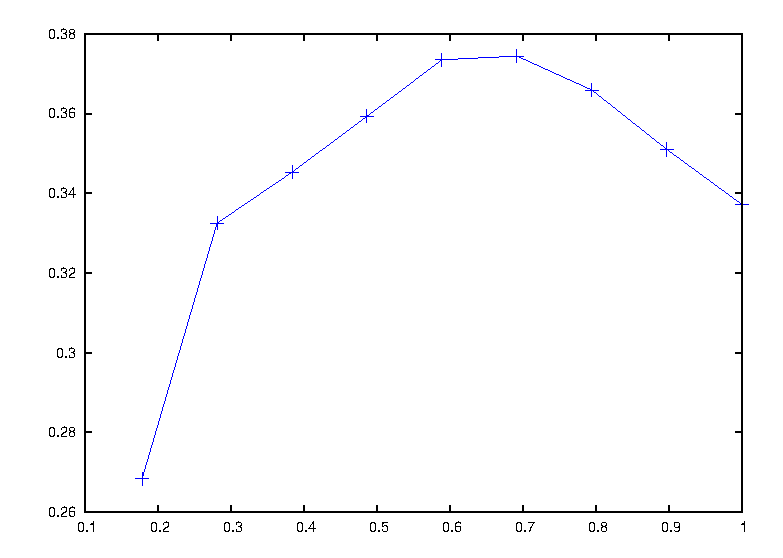
\includegraphics[width=\textwidth]{figures/alphaomega-1.eps}
  \end{minipage} 
  \hfill
  \begin{minipage}[t]{0.49\textwidth}
  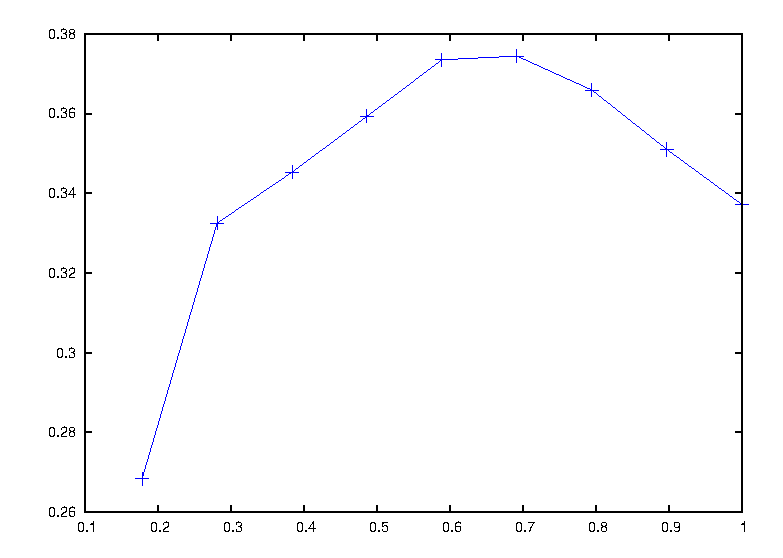
\includegraphics[width=\textwidth]{figures/alphaomega-2.eps}
  \end{minipage}
  \caption{Plot of $\alpha^\omega_P\alpha^\omega_D$ for 9 values 
           of $\omega \in [\alpha_P\alpha_D, 1]$
           in two iterations of problem {\tt capri}.}
  \label{fig:alphaomega}
\end{figure}


%
% Section
%
\section{Numerical results}
\label{sec:NumericalResults}

We have implemented our proposal within the \HOPDM interior point solver 
\cite{HOPDM}, and tested it in a series of computational 
experiments, using test problems from different collections. 
As a comparison, we present the results obtained by \PCx \cite{PCx}, 
a reference implementation of interior point methods.
The two implementations, \PCx and \HOPDM, have different termination criteria 
in their default configurations. For the purpose of consistency,
in the results shown, 
we decided to implement in \HOPDM the criteria used by \PCx.
Therefore, for all solvers optimal termination occurs when the conditions
(\ref{eq:TerminationCriteriaPCx}) are met, with feasibility
accuracy $p=8$ and complementarity accuracy $q = 10$.

We use $\gamma = 0.1$ in the definition of the symmetric 
neighbourhood and define aspiration levels for the stepsizes using the rule
\[
  \tilde{\alpha}_{P} = \min(1.5 \alpha_{P} \! + \! 0.3, \, 1) 
  \quad \mbox{ and } \quad
  \tilde{\alpha}_{D} = \min(1.5 \alpha_{D} \! + \! 0.3, \, 1). 
\]
The values suggested in \cite{Gondzio96} were more conservative:
$\tilde{\alpha} = \min (\alpha + 0.1, \, 1)$.
Thanks to the weighting mechanism we can control 
the contribution of the corrector in an adaptive way,
and thus be more demanding in our definition of aspired stepsizes.

Centrality correctors are accepted in the primal and/or dual space
if ${\alpha}_{P}^{new} \geq 1.01 \alpha_{P}$ 
and/or ${\alpha}_{D}^{new} \geq 1.01 \alpha_{D}$, respectively.
Note that this is different from what is described in \cite{Gondzio96}, where
a corrector is accepted if ${\alpha}^{new} \geq \alpha + 0.1\delta$, 
for an aspiration level $\delta = 0.1$.

We implemented a simple linesearch procedure to locate $\hat\omega$.
We choose 9 points uniformly spaced in the interval
$[\alpha_P\alpha_D, 1]$ and evaluate, for each of these points,
the stepsizes $\alpha^\omega_P$ and $\alpha^\omega_D$ in both spaces. 
When a larger stepsize $\alpha^\omega_P$ or $\alpha^\omega_D$ is obtained, 
the corresponding $\omega$ is stored as $\omega_P$ or $\omega_D$ 
respectively. Hence, in our implementation we allow different
weightings for directions in the primal and dual spaces.

We present our results in terms of number of iterations and number 
of backsolve operations. The rationale behind this decision is that 
the multiple centrality correctors technique determines the number 
of allowed correctors on the basis of the ratio between factorisation 
cost and backsolve cost. This ratio can be very different across 
implementations, and is mainly influenced by the linear algebra 
routines used. 
\HOPDM comes with an in-house linear algebra implementation, while
\PCx relies on the more sophisticated sparse Cholesky solver
of Ng and Peyton. Therefore, the \PCx code tends to use less 
correctors per iteration.
In all other respects, the correction scheme closely follows the one
of \HOPDM and the paper \cite{Gondzio96}.

%
%
\subsection{Comparison with Mehrotra and Li's approach}
\label{ML-tests}

We first considered the test set used in \cite{MehrotraLi}.
It contains 101 problems from the Netlib and Kennington collections. 
We will refer to is as Mehrotra and Li's test collection.
In Table~\ref{MLtotals} we present the computational comparison 
outlining the total number of iterations and the total number 
of backsolves necessary to solve the problems in this test set. 
Column \HO\ displays the results obtained
by the previous implementation of \HOPDM, while column d\HO\ reports
the results obtained by the current implementation of weighted
correctors with a default choice of the number of centrality correctors. 
The last column presents the relative change between the two 
versions of \HOPDM tested. 
As a reference, we also report in this table the overall
statistics of \PCx (release 1.1) on these problems.
We found the number of backsolves by counting the number of calls 
to the functions {\tt IRSOLV()} and {\tt EnhanceSolve()}, for \HOPDM and
\PCx respectively.
%
\begin{table}[ht]
  \centering
  \begin{tabular}{|l|c||c|c|r|}\cline{2-5}
    \multicolumn{1}{c|}{}&\PCx & \HO& d\HO&\multicolumn{1}{c|}{Change}\\ \hline
    Iterations       & 2114 & 1871  & 1445           &   -22.77\% \\ 
    Backsolves       & 4849 & 6043  & 5717           &   -5.39\%  \\
    Backsolves/iter. & 2.29 & 3.23  & 3.95           &   +22.29\% \\ \hline
  \end{tabular}
  \caption{Overall results obtained on Mehrotra and Li's test collection.}
  \label{MLtotals}
\end{table}
%
\\From Table~\ref{MLtotals} we first observe the very small number 
of backsolves per iteration needed by \PCx. This is due to the fact 
that \PCx allows the use of Gondzio's multiple centrality correctors 
only in 4 problems: {\tt dfl001}, {\tt maros-r7}, {\tt pds-10} and 
{\tt pds-20}.
%
Also we notice that when we allow an adaptive weighting 
of the correctors there is a tendency to use more correctors 
per iteration than previously. 
This happens because the weighting mechanism makes it more likely
to accept some correctors that would otherwise have been rejected
as too aggressive.
While this usually leads to a decrease 
in iteration count, it also makes each iteration more expensive,
as more backsolves are performed.

In Table~\ref{TimeML} we detail the problems for which we obtained savings 
in computational time. Given the small dimension of most of the problems 
in the Netlib collection, we did not expect major savings. However, as the
problem sizes increase, we can see that the proposed way of evaluating and
weighting the correctors pays off. This led us to investigate further 
the performance of the proposed implementation, which we will discuss
in Section~\ref{BN-tests}.
%
\begin{table}[ht]
  \centering
  \begin{minipage}[t]{0.36\textwidth}
    \begin{tabular}{|l|r|r|}\hline
      Problem & \multicolumn{1}{c|}{\HO} & \multicolumn{1}{c|}{d\HO} \\ \hline
      bnl1    &   0.36 &   0.25 \\
      d{f}l001& 150.63 & 114.80 \\
      maros-r7&   7.76 &   7.52 \\
      pilot   &   5.23 &   4.35 \\ \hline
    \end{tabular}
  \end{minipage}
  \begin{minipage}[t]{0.36\textwidth}
    \begin{tabular}{|l|r|r|}\hline
      Problem & \multicolumn{1}{c|}{\HO} & \multicolumn{1}{c|}{d\HO} \\ \hline
      pilot87 &  12.62 &  11.88 \\ 
      pds-06  &  24.59 &  21.31 \\
      pds-10  &  96.57 &  79.29 \\
      pds-20  & 923.71 & 633.64 \\ \hline
    \end{tabular}
  \end{minipage}
  \caption{Problems that showed time savings (times are in seconds).}
  \label{TimeML}
\end{table}

%In terms of the number of iterations, Mehrotra and Li's scheme is extremely 
%promising. 
% However, only 13 problems out of 101 showed a reduction 
% in computing time when using 4 Krylov directions. 
%
We were particularly interested in comparing the results produced by our 
weighted correctors approach with those obtained by the subspace search
scheme of Section~\ref{sec:MehrotraLi} and published in \cite{MehrotraLi}. 
In the tables of results presented in \cite{MehrotraLi}, the best 
performance in terms of iteration count is obtained by \PCx-4, which 
uses 4 Krylov subspace vectors. These directions are combined with 
an affine-scaling predictor direction and Mehrotra's second-order 
correction, leading to 6 backsolves per iteration. 
%  {\bf (but it's not clear that they use Krylov 
%        directions and solve a linear subproblem at every iteration)}
This number increases when the linear subproblem produces an optimal 
objective value smaller than a specified threshold or the new iterate 
fails to satisfy some neighbourhood condition. In these cases 
the pure centering direction $\Delta_\mu w$ also needs to be computed,
and a seventh backsolve is performed.

In Table~\ref{MLresults} we present a full comparison of the
weighted correctors and Mehrotra and Li's strategies.
In columns \HO-0 and \HO-4, we present 
the results obtained by \HOPDM when forcing the use of 0 and 4 
multiple centrality correctors. 
In the column called \HO-$\infty$ we report the results 
obtained when an unlimited number of correctors is allowed
(in practice we allow no more than 20 correctors).
The last column, labelled d\HO, presents the results obtained 
by the default way of choosing the number of correctors allowed.
As we understand the paper \cite{MehrotraLi}, \PCx-0 uses exactly 
2 backsolves per iteration: one to compute the affine-scaling direction,
another to compute Mehrotra's corrector; \PCx-4 computes
four additional Krylov vectors, hence it uses
6 backsolves per iteration.
Consequently, up to 2 and 6 backsolves per iteration are allowed
in \PCx-0 and \PCx-4 and in \HO-0 and \HO-4, respectively.

The number of backsolves reported for \HOPDM includes two needed by 
the initialisation procedure: the number of backsolves 
should not exceed $2 \times {\rm Its} + 2$, 
and $6 \times {\rm Its} + 2$ respectively
for \HO-0 and \HO-4, where {\rm  Its} is the number of iterations.
The observed number of backsolves is often much smaller
than these bounds because the correcting mechanism switches off 
when the stepsizes are equal to 1 or when the corrector does not 
improve the stepsize. Problem {\tt afiro} solved by \HO-4 needs 24 
backsolves, 22 of which compute different components of directions, 
hence the average number of backsolves per iteration is only 22/6 
and is much smaller than 6. Occasionally,
as a consequence of numerical errors, certain components 
of direction are rejected on the grounds of insufficient accuracy.
In such cases, the number of backsolves may exceed the stated upper bounds.
The reader may observe, for example, that {\tt pilot4} is solved by \HO-4
in 16 iterations, but the number of backsolves is equal to 100 and 
exceeds $6 \times 16 + 2 = 98$.

The version \HO-$\infty$ requires 1139 iterations to solve 
the collection of 101 problems, an average of just above 11 iterations
per problem. This version has only an academic interest, 
yet it reveals a spectacular efficiency of interior point 
methods which can solve difficult linear programs of medium sizes 
(reaching a couple of hundred thousand variables) in just 
a few iterations.
In particular, it suggests that if we had a cheap way of generating
search directions, then it would be beneficial to have as many as possible.

%
%
\subsection{Larger test problems}
\label{BN-tests}

We have applied our algorithm to examples from other test collections 
besides Netlib.
We used a collection of medium to large problems taken from different
sources. Problems {\tt CH} through {\tt CO9}
are MARKAL (market allocation) models; {\tt mod2} through {\tt worldl} are
agricultural models used earlier in \cite{Gondzio96}; problems {\tt route}
through {\tt rlfdual} can be retrieved from 
\begin{center}
{\tt http://www.sztaki.hu/\~{}meszaros/public\_ftp/lptestset/misc/},
\end{center}
and problems {\tt neos1} through {\tt fome13} can be retrieved from 
\begin{center}
{\tt ftp://plato.asu.edu/pub/lptestset/}.
\end{center}

In Table~\ref{TimeBN} we detail the sizes of these problems and provide 
a time comparison between our previous implementation (shown in column
\HO), and the current one (in column d\HO).
This test collection contains problems large enough 
to show a consistent improvement in CPU time. 
We only recorded a deterioration of the performance by more than 1 second
in 4 problems ({\tt mod2}, {\tt dbc1}, {\tt watson-1}, {\tt sgpf5y6}).
The improvements are significant on problems with a large 
number of nonzero elements. In these cases, d\HO\
produces savings ranging from about 10\% to 30\%, with remarkable results
in {\tt rail2586} and {\tt rail4284}, for which the relative savings 
reach 45\% and 65\%, respectively.

In Figure~\ref{fig:PerfProfile}, we show the CPU-time based 
performance profile \cite{DolanMore} for the two algorithms. 
This graph shows the proportion of problems that each algorithm
has solved within $\tau$ times of the best. Hence, for
$\tau = 1$ it indicates that d\HO\ has been the best solver on 72\%
of the problems, against 28\% for \HO. For larger values of $\tau$,
the performance profile for d\HO\ stays above the one for \HO, thus
confirming its superiority. In particular, d\HO solves all problems
within 1.3 times of the best.

\begin{figure}[ht]
  \centering
  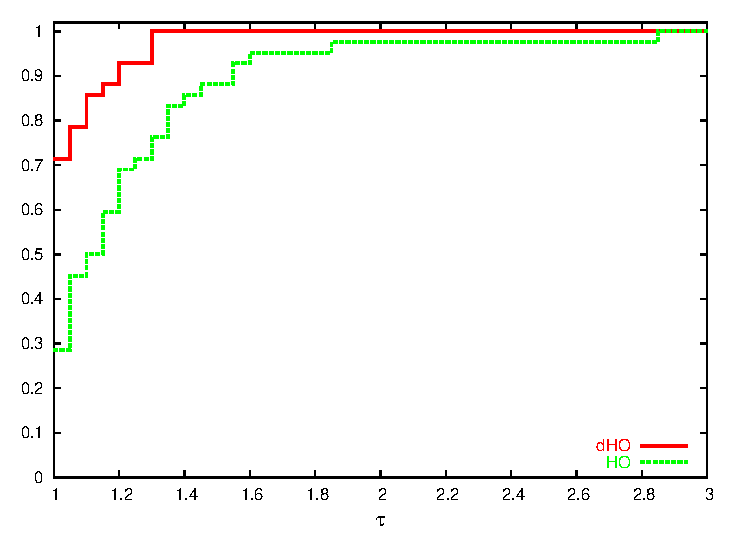
\includegraphics[width=0.75\textwidth]{figures/perfprof-BN.eps}
  \caption{Performance profiles for \HO (dashed) and d\HO (solid)
           on the set of problems of Table~\ref{TimeBN}.}
  \label{fig:PerfProfile}
\end{figure}

More numerical results obtained on some collections of stochastic
programming problems and quadratic problems can be found in
\cite{ColomboGondzio05}.

\newpage

%
% Section
%
\section{Tables of results}

% shrink the spacing of the columns for the following tables
\setlength{\tabcolsep}{4.6pt}

%
%
\subsection*{Mehrotra and Li's test collection}

\begin{small}
\begin{longtable}{|l|r|rr||r|rr||rr||rr|} \hline 
\raisebox{-1.5ex}[0ex][-1.5ex]{Problem} & \multicolumn{1}{c|}{PCx0}
        & \multicolumn{2}{c||}{HO-0}
        & \multicolumn{1}{c|}{PCx4} 
        & \multicolumn{2}{c||}{HO-4} 
        & \multicolumn{2}{c||}{HO\raisebox{1pt}{-$\infty$}} 
        & \multicolumn{2}{c|}{dHO} \\ \cline{2-11}
        & Its
        & Its & Bks
        & Its
        & Its & Bks
        & Its & Bks
        & Its & Bks \\ \hline
\endhead
\hline
\multicolumn{11}{c}{\raisebox{-1ex}{Table~\ref{MLresults}:
Comparison with Mehrotra and Li's algorithm.}}
\endfoot
\label{MLresults}
25fv47 & 25 & 27 & 55 & 15 & 15 & 95 & 14 & 184 & 18 & 76 \\
80bau3b & 36 & 31 & 64  & 22 & 15 & 93 & 13 & 195 & 18 & 78 \\
adlittle & 11 & 12 & 25  & 8 & 9 & 47 & 9 & 91 & 10 & 29 \\
afiro & 7 & 8 & 13  & 6 & 6 & 24 & 6 & 35 & 7 & 15 \\
agg & 18 & 21 & 43  & 10 & 13 & 79 & 12 & 143 & 14 & 57 \\
agg2 & 22 & 22 & 46  & 15 & 14 & 86 & 12 & 151 & 15 & 61 \\
agg3 & 21 & 20 & 41  & 14 & 15 & 84 & 14 & 147 & 15 & 62 \\
bandm & 17 & 14 & 30  & 11 & 10 & 58 & 9 & 106 & 11 & 34 \\
beaconfd & 10 & 10 & 19  & 7 & 8 & 40 & 9 & 82 & 8 & 23 \\
blend & 9 & 10 & 20  & 7 & 8 & 42 & 8 & 61 & 8 & 23 \\
bnl1 & 36 & 39 & 80  & 27 & 17 & 107 & 17 & 162 & 25 & 91 \\
bnl2 & 32 & 25 & 51  & 19 & 16 & 93 & 13 & 171 & 16 & 93 \\
boeing1 & 20 & 20 & 40  & 12 & 13 & 76 & 11 & 142 & 15 & 47 \\
boeing2 & 12 & 14 & 28  & 10 & 11 & 61 & 10 & 117 & 12 & 34 \\
bore3d & 15 & 15 & 28  & 11 & 11 & 60 & 10 & 102 & 12 & 33 \\
brandy & 19 & 19 & 38  & 13 & 14 & 82 & 12 & 160 & 17 & 50 \\
capri & 18 & 19 & 38  & 12 & 11 & 63 & 11 & 121 & 14 & 43 \\
cycle & 23 & 27 & 55  & 13 & 18 & 104 & 15 & 165 & 19 & 83 \\
czprob & 27 & 23 & 46  & 16 & 14 & 82 & 13 & 176 & 19 & 60 \\
d2q06c & 29 & 31 & 64  & 18 & 17 & 105 & 14 & 201 & 17 & 106 \\
d6cube & 19 & 17 & 35  & 11 & 12 & 64 & 11 & 139 & 12 & 64 \\
degen2 & 12 & 14 & 29  & 8 & 10 & 62 & 9 & 100 & 11 & 44 \\
degen3 & 16 & 20 & 42  & 10 & 14 & 84 & 11 & 121 & 14 & 84 \\
df{l}001 & 47 & 46 & 97 & 31 & 26 & 152 & 25 & 329 & 22 & 222 \\
e226 & 17 & 19 & 40  & 11 & 14 & 87 & 12 & 132 & 16 & 49 \\
etamacro & 23 & 20 & 42  & 14 & 12 & 73 & 12 & 141 & 13 & 52 \\
{f}f{f}f{f}800 & 27 & 30 & 62  & 16 & 17 & 108 & 17 & 244 & 19 & 84 \\
finnis & 23 & 21 & 42  & 14 & 29 & 169 & 17 & 197 & 26 & 81 \\
fit1d & 17 & 16 & 34  & 11 & 12 & 75 & 11 & 148 & 15 & 47 \\
fit1p & 17 & 18 & 38  & 12 & 12 & 72 & 11 & 156 & 15 & 47 \\
fit2d & 22 & 29 & 60  & 12 & 17 & 107 & 12 & 160 & 24 & 83 \\
fit2p & 20 & 24 & 49  & 12 & 15 & 90 & 12 & 150 & 17 & 54 \\
forplan & 22 & 19 & 39  & 13 & 13 & 80 & 13 & 145 & 15 & 46 \\
ganges & 19 & 12 & 26  & 11 & 8 & 50 & 8 & 93 & 10 & 32 \\
gfrd-pnc & 18 & 14 & 27  & 11 & 9 & 53 & 8 & 91 & 11 & 32 \\
greenbea & 36 & 37 & 76  & 28 & 23 & 146 & 20 & 263 & 22 & 98 \\
greenbeb & 32 & 41 & 84 & 25 & 22 & 139 & 19 & 242 & 28 & 99 \\
grow15 & 18 & 11 & 22  & 13 & 8 & 50 & 7 & 94 & 9 & 26 \\
grow22 & 21 & 11 & 22  & 15 & 8 & 49 & 7 & 66 & 9 & 28 \\
grow7 & 15 & 11 & 22  & 11 & 8 & 46 & 7 & 57 & 9 & 26 \\
israel & 19 & 21 & 44  & 12 & 13 & 81 & 11 & 135 & 16 & 52 \\
kb2 & 12 & 12 & 24  & 8 & 9 & 47 & 8 & 75 & 10 & 29 \\
lotfi & 14 & 14 & 28  & 9 & 9 & 47 & 9 & 77 & 11 & 31 \\
maros-r7 & 17 & 15 & 30  & 11 & 11 & 62 & 9 & 114 & 10 & 68 \\
maros & 19 & 20 & 41 & 12 & 13 & 79 & 11 & 136 & 16 & 51 \\
nesm & 25 & 27 & 56  & 17 & 14 & 87 & 12 & 153 & 17 & 72 \\
perold & 32 & 24 & 49  & 21 & 14 & 87 & 13 & 172 & 16 & 69 \\
pilot & 36 & 27 & 56  & 22 & 15 & 95 & 14 & 170 & 15 & 95 \\
pilot4 & 68 & 30 & 62  & 53 & 16 & 100 & 17 & 228 & 19 & 84 \\
pilotja & 29 & 30 & 62  & 21 & 15 & 95 & 14 & 179 & 16 & 84 \\
pilotnov & 17 & 15 & 30 & 11 & 10 & 53 & 9 & 87 & 10 & 46 \\
pilotwe & 48 & 30 & 62 & 27 & 15 & 94 & 15 & 204 & 19 & 83 \\
pilot87 & 34 & 31 & 64 & 19 & 16 & 99 & 14 & 220 & 15 & 125 \\
recipe & 9 & 8 & 15  & 7 & 7 & 35 & 7 & 49 & 7 & 18 \\
scagr25 & 16 & 16 & 32  & 11 & 9 & 52 & 8 & 92 & 11 & 35 \\
scagr7   & 14 & 12 & 23  & 9 & 10 & 56 & 9 & 82 & 11 & 32 \\
scfxm1   & 18 & 17 & 35  & 11 & 10 & 63 & 9 & 112 & 14 & 43 \\
scfxm2   & 19 & 19 & 40  & 12 & 11 & 70 & 10 & 140 & 15 & 46 \\
scfxm3   & 21 & 19 & 40  & 12 & 12 & 73 & 10 & 128 & 15 & 47 \\
scrs8    & 21 & 17 & 35  & 13 & 11 & 72 & 10 & 112 & 13 & 40 \\
scsd1    &  9 &  8 & 15  & 7 & 7 & 30 & 7 & 54 & 7 & 18 \\
scsd6    & 12 & 10 & 20  & 9 & 8 & 41 & 8 & 68 & 9 & 24 \\
scsd8    & 12 & 11 & 21  & 8 & 7 & 33 & 7 & 60 & 9 & 23 \\
sctap1   & 16 & 17 & 33  & 9 & 11 & 58 & 11 & 114 & 13 & 37 \\
sctap2   & 13 & 15 & 29  & 9 & 10 & 51 & 8 & 86 & 12 & 33 \\
sctap3   & 13 & 15 & 30  & 10 & 11 & 51 & 8 & 87 & 12 & 33 \\
seba     & 14 &  9 & 15  & 9 & 7 & 33 & 7 & 114 & 8 & 19 \\
share1b  & 19 & 21 & 43  & 12 & 13 & 82 & 12 & 129 & 17 & 54 \\
share2b  & 17 & 15 & 29  & 12 & 9 & 43 & 8 & 72 & 12 & 35 \\
shell    & 20 & 21 & 42  & 13 & 12 & 73 & 10 & 128 & 14 & 44 \\
ship04l  & 12 & 11 & 24  & 8 & 8 & 49 & 8 & 118 & 10 & 31 \\
ship04s  & 13 & 12 & 26  & 8 & 9 & 53 & 8 & 104 & 10 & 31 \\
ship12l  & 14 & 13 & 28  & 11 & 8 & 47 & 8 & 103 & 11 & 34 \\
ship12s  & 12 & 14 & 29  & 8 & 9 & 51 & 8 & 102 & 11 & 34 \\
sierra   & 19 & 18 & 38  & 11 & 11 & 66 & 10 & 104 & 14 & 43 \\
stair    & 14 & 18 & 36  & 11 & 16 & 91 & 11 & 145 & 12 & 46 \\
standata & 13 & 16 & 30  & 8 & 12 & 61 & 10 & 117 & 13 & 35 \\
standmps & 22 & 21 & 40  & 16 & 14 & 78 & 13 & 147 & 16 & 46 \\
stocfor1 & 11 & 12 & 22  & 7 & 8 & 43 & 8 & 77 & 9 & 26 \\
stocfor2 & 20 & 19 & 38  & 13 & 12 & 74 & 10 & 151 & 15 & 46 \\
truss    & 20 & 17 & 35  & 12 & 10 & 61 & 9 & 113 & 11 & 46 \\
tuff     & 19 & 15 & 30  & 12 & 9 & 51 & 9 & 98 & 10 & 39 \\
vtpbase  & 11 & 11 & 20  & 7 & 9 & 40 & 8 & 103 & 9 & 25 \\
wood1p   & 19 & 22 & 43  & 14 & 14 & 85 & 13 & 162 & 16 & 65 \\
woodw    & 30 & 29 & 59  & 19 & 16 & 99 & 14 & 167 & 18 & 77 \\
cre-a    & 24 & 25 & 52  & 15 & 15 & 97 & 12 & 143 & 18 & 59 \\
cre-b    & 40 & 42 & 86  & 23 & 24 & 148 & 16 & 219 & 22 & 99 \\
cre-c    & 25 & 28 & 57  & 15 & 16 & 98 & 14 & 184 & 19 & 63 \\
cre-d    & 39 & 43 & 88  & 26 & 22 & 137 & 17 & 233 & 22 & 100 \\
ken-07   & 15 & 12 & 25  & 10 & 8 & 48 & 7 & 107 & 10 & 31 \\
ken-11   & 21 & 15 & 32  & 13 & 10 & 63 & 9 & 133 & 13 & 40 \\
ken-13   & 28 & 19 & 40  & 16 & 11 & 69 & 11 & 138 & 15 & 47 \\
ken-18   & 30 & 24 & 49  & 21 & 13 & 78 & 9 & 139 & 15 & 63 \\
osa-07   & 18 & 23 & 47  & 12 & 13 & 73 & 11 & 111 & 13 & 41 \\
osa-14   & 19 & 19 & 39  & 18 & 12 & 73 & 11 & 106 & 15 & 47 \\
osa-30   & 24 & 20 & 40  & 18 & 15 & 93 & 13 & 147 & 17 & 60 \\
osa-60   & 22 & 20 & 41  & 15 & 12 & 70 & 11 & 118 & 14 & 46 \\
pds-02   & 25 & 19 & 38  & 15 & 14 & 77 & 11 & 124 & 15 & 60 \\
pds-06   & 35 & 27 & 56  & 23 & 17 & 100 & 15 & 177 & 17 & 118 \\
pds-10   & 41 & 32 & 66 & 27 & 20 & 120 & 18 & 199 & 18 & 155 \\
pds-20   & 58 & 48 & 98 & 34 & 23 & 136 & 21 & 253 & 21 & 198 \\ \hline
Totals & 2,194& 2,047& 4,169& 1,438& 1,289& 7,608& 1,139& 13,699& 1,445& 5,717
\end{longtable} 
\end{small}

%
%
\subsection*{Other large LP problems}

\begin{small}
\begin{longtable}{|l|rrr|r|r|r|} \hline 
  \multicolumn{1}{|c|}{\normalsize Problem}
& \multicolumn{1}{c}{\normalsize Rows}
& \multicolumn{1}{c}{\normalsize Columns}
& \multicolumn{1}{c|}{\normalsize Nonzeros}
& \multicolumn{1}{c|}{\normalsize \HO}
& \multicolumn{1}{c|}{\normalsize d\HO}
& \multicolumn{1}{c|}{\normalsize Change}\\ \hline
\endhead
\hline
\multicolumn{7}{c}{\normalsize \raisebox{-1ex}{Table~\ref{TimeBN}: 
Time comparison on larger problems (times are in seconds).}}
\endfoot
\label{TimeBN}
CH       &   3,852 &    5,062 &    42,910 &    1.03 &    1.23 &  19.4\% \\
GE       &  10,339 &   11,098 &    53,763 &    5.72 &    5.46 &  -4.5\% \\
NL       &   7,195 &    9,718 &   102,570 &    4.37 &    3.95 &  -9.6\% \\
BL       &   6,325 &    8,018 &    58,607 &    2.15 &    2.14 &  -0.5\% \\
BL2      &   6,325 &    8,018 &    58,607 &    2.35 &    2.31 &  -1.7\% \\
UK       &  10,131 &   14,212 &   128,341 &    2.48 &    3.21 &  29.4\% \\
CQ5      &   5,149 &    7,530 &    83,564 &    2.54 &    2.60 &   2.4\% \\
CQ9      &   9,451 &   13,778 &   157,598 &    9.67 &    8.84 &  -8.6\% \\
CO5      &   5,878 &    7,993 &    92,788 &    3.16 &    3.59 &  13.6\% \\
CO9      &  10,965 &   14,851 &   176,346 &   21.10 &   15.35 & -27.3\% \\
mod2     &  35,664 &   31,728 &   220,116 &   20.59 &   21.68 &   5.3\% \\
world    &  35,510 &   32,734 &   220,748 &   26.35 &   23.41 & -11.2\% \\
world3   &  36,266 &   33,675 &   224,959 &   31.13 &   27.49 & -11.7\% \\
world4   &  52,996 &   37,557 &   324,502 &   73.21 &   56.14 & -23.3\% \\
world6   &  47,038 &   32,670 &   279,024 &   39.33 &   32.79 & -16.6\% \\
world7   &  54,807 &   37,582 &   333,509 &   43.14 &   36.02 & -16.5\% \\
worldl   &  49,108 &   33,345 &   291,942 &   43.95 &   36.82 & -16.2\% \\
route    &  20,894 &   23,923 &   210,025 &   40.92 &   33.78 & -17.4\% \\
ulevi    &   6,590 &   44,605 &   162,207 &    9.04 &    9.55 &   5.6\% \\
ulevimin &   6,590 &   44,605 &   162,207 &   16.52 &   16.46 &  -0.4\% \\
dbir1    &  18,804 &   27,355 & 1,067,815 &  162.18 &  146.51 &  -9.7\% \\
dbir2    &  18,906 &   27,355 & 1,148,847 &  208.93 &  156.11 & -25.3\% \\
dbic1    &  43,200 &  183,235 & 1,217,046 &   72.96 &   77.31 &   5.9\% \\
pcb1000  &   1,565 &    2,428 &    22,499 &    0.26 &    0.33 &  26.9\% \\
pcb3000  &   3,960 &    6,810 &    63,367 &    1.13 &    1.16 &   2.7\% \\
rlfprim  &  58,866 &    8,052 &   265,975 &   15.63 &   15.08 &  -3.5\% \\
rlfdual  &   8,052 &   66,918 &   328,891 &   71.17 &   49.79 & -30.0\% \\
neos1    & 131,581 &    1,892 &   468,094 &  169.11 &  141.89 & -16.1\% \\
neos2    & 132,568 &    1,560 &   552,596 &  113.86 &   86.13 & -24.4\% \\
neos3    & 132,568 &    1,560 &   552,596 &  132.02 &  120.59 &  -8.7\% \\
neos     & 479,119 &   36,786 & 1,084,461 &1,785.80 &1,386.58 & -22.4\% \\
watson-1 & 201,155 &  383,927 & 1,053,564 &  138.60 &  166.21 &  19.9\% \\
sgpf5y6  & 246,077 &  308,634 &   902,275 &   49.58 &   64.45 &  30.0\% \\
stormG2-1000 & 528,185 & 1,259,121 & 4,228,817 & 1,661.54 & 1,623.19 & -2.3\%\\
rail507  &     507 &   63,009 &   472,358 &    9.77 &   10.10 &   3.4\% \\
rail516  &     516 &   47,311 &   362,207 &    7.59 &    5.89 & -22.4\% \\
rail582  &     582 &   55,515 &   457,223 &    9.67 &    9.60 &  -0.7\% \\
rail2586 &   2,586 &  920,683 & 8,929,459 &1,029.36 &  566.82 & -44.9\% \\
rail4284 &   4,284 &1,092,610 &12,372,358 &2,779.63 &  978.48 & -64.8\% \\
fome11   &  12,142 &   24,460 &    83,746 &  407.20 &  265.21 & -34.9\% \\
fome12   &  24,284 &   48,920 &   167,492 &  766.96 &  508.61 & -33.7\% \\
fome13   &  48,568 &   97,840 &   334,984 & 1,545.05 & 990.62 & -35.9\% \\
\end{longtable} 
\end{small}

\ignore{
\begin{small}
\begin{longtable}{|l|rr|rr|rr|rr|} \hline 
\raisebox{-1.5ex}[0ex][-1.5ex]{Problem}
& \multicolumn{2}{c|}{HO-0}
& \multicolumn{2}{c|}{HO-4} 
& \multicolumn{2}{c|}{HO\raisebox{1pt}{-$\infty$}} 
& \multicolumn{2}{c|}{dHO} \\ \cline{2-9}
& Its & Bks
& Its & Bks
& Its & Bks
& Its & Bks \\ \hline
\endhead
\hline
\multicolumn{9}{c}{\raisebox{-1ex}{Table~\ref{BNresults}: Comparison on 
    large problems.}}
\endfoot
\label{BNresults}
CH & 26 & 54 & 15 & 94 & 12 & 155 & 16 & 83 \\
GE & 39 & 80 & 20 & 127 & 23 & 307 & 20 & 133 \\
NL & 32 & 66 & 15 & 93 & 13 & 192 & 15 & 93 \\
BL & 28 & 58 & 15 & 93 & 13 & 182 & 16 & 85 \\
BL2 & 32 & 66 & 15 & 94 & 13 & 189 & 16 & 85 \\
UK & 30 & 62 & 15 & 93 & 14 & 191 & 19 & 82 \\
CQ5 & 41 & 84 & 22 & 135 & 18 & 253 & 24 & 109 \\
CQ9 & 49 & 100 & 24 & 154 & 22 & 299 & 26 & 152 \\
CO5 & 50 & 102 & 28 & 179 & 36 & 472 & 30 & 142 \\
CO9 & 58 & 118 & 62 & 357 & 52 & 627 & 41 & 237 \\
mod2 & 38 & 78 & 21 & 128 & 15 & 248 & 22 & 121 \\
world & 42 & 86 & 21 & 128 & 16 & 230 & 22 & 121 \\
world3 & 52 & 106 & 28 & 172 & 19 & 291 & 28 & 158 \\
world4 & 51 & 104 & 27 & 164 & 21 & 281 & 26 & 170 \\
world6 & 44 & 90 & 23 & 144 & 19 & 261 & 22 & 145 \\
world7 & 40 & 82 & 22 & 135 & 17 & 267 & 21 & 137 \\
worldl & 52 & 106 & 25 & 156 & 20 & 282 & 24 & 157 \\
route & 21 & 42 & 14 & 80 & 11 & 114 & 14 & 80 \\
ulevi & 26 & 51 & 17 & 103 & 15 & 185 & 17 & 103 \\
ulevimin & 68 & 138 & 27 & 172 & 22 & 306 & 27 & 186 \\
dbir1 & 22 & 44 & 13 & 80 & 9 & 112 & 12 & 104 \\
dbir2 & 25 & 52 & 13 & 81 & 12 & 167 & 11 & 104 \\
dbic1 & 54 & 109 & 20 & 128 & 17 & 213 & 24 & 109 \\
pcb1000 & 20 & 42 & 12 & 74 & 11 & 138 & 15 & 62 \\
pcb3000 & 23 & 48 & 13 & 80 & 12 & 165 & 15 & 63 \\
rlfprim & 13 & 25 & 8 & 40 & 7 & 65 & 8 & 40 \\
rlfdual & 13 & 25 & 9 & 49 & 9 & 80 & 9 & 63 \\
neos1 & 55 & 111 & 29 & 179 & 21 & 275 & 24 & 195 \\
neos2 & 40 & 81 & 24 & 140 & 19 & 210 & 19 & 125 \\
neos3 & 49 & 98 & 35 & 191 & 30 & 326 & 28 & 195 \\
neos & 109 & 220 & 41 & 260 & 41 & 591 & 49 & 430 \\
watson-1 & 112 & 226 & 30 & 192 & 46 & 655 & 49 & 195 \\
sgpf5y6 & 45 & 92 & 24 & 157 & 19 & 214 & 30 & 109 \\
stormG2-1000 & 130 & 261 & 66 & 398 & 53 & 687 & 73 & 316 \\
rail507 & 35 & 71 & 15 & 91 & 14 & 199 & 19 & 81 \\
rail516 & 30 & 61 & 12 & 67 & 10 & 142 & 15 & 56 \\
rail582 & 45 & 92 & 16 & 102 & 19 & 229 & 19 & 84 \\
rail2586 & 99 & 200 & 24 & 147 & 20 & 287 & 24 & 149 \\
rail4284 & 65 & 132 & 25 & 158 & 22 & 361 & 19 & 213 \\
fome11 & 44 & 92 & 25 & 150 & 23 & 294 & 24 & 224 \\
fome12 & 44 & 91 & 25 & 147 & 20 & 286 & 22 & 215 \\
fome13 & 43 & 91 & 24 & 145 & 20 & 289 & 20 & 215 \\ \hline
   Totals & 1,934 & 3,937 & 959 & 5,857 & 845 & 11,317 & 974 & 5,926
\end{longtable} 
\end{small}
}
\setlength{\tabcolsep}{6pt}
